\chapter*{Introduction} % Main chapter title
\addcontentsline{toc}{chapter}{Introduction}  

%Le but de l'avant-propos est d'améliorer les conditions dans lesquelles les membres d’un jury, vont pouvoir l’apprécier.
%C’est une partie facultative du travail de recherche dans laquelle l’auteur peut expliquer les raisons qui l’ont incité à étudier le sujet en question, tout en exposant le but poursuivi et les difficultés rencontrées en cours de recherche.

C'est au sein du ministère  du travail, de la santé et des solidarités, à la Direction de la Sécurité Sociale que j'ai choisi d'effectuer mon alternance de Master 2 ISF.

A la date de remise de mon mémoire, la Direction de la Sécurité Sociale est sous l’autorité conjointe de la ministre démissionnaire du Travail, de la Santé et des Solidarités, Mme Catherine VAUTRIN et du ministre démissionnaire de l’Économie, des Finances et de la Souveraineté industrielle et numérique, M. Bruno LEMAIRE. 
La Direction de la Sécurité Sociale est organisée en plusieurs sous directions. C’est au sein de la troisième sous direction en charge des retraites et des institutions de la protection sociale complémentaire que j’ai pu effectuer mon alternance. Cette sous-direction est organisée en trois bureaux, ayant respectivement la charge des régimes de base (bureau 3A), des régimes spéciaux (bureau 3B) et des régimes professionnels de retraite et institutions de protection sociale complémentaire (bureau 3C).

La sous-directrice actuellement en charge de la troisième sous direction est Delphine CHAUMEL. Son adjoint et ancien chef du bureau 3C est Hédi BRAHIMI.
C’est au sein du pôle Data Science et Actuariat du bureau 3C que j’ai effectué mon alternance, accompagné par Taha BENABDELAZIZ, mon tuteur d'alternance et chef du pôle.
Le chef de ce bureau est en cours de recrutement, et les deux adjoints au chef sont Rémi TABAUD-DEBOTH, en charge du pôle Protection Sociale Complémentaire et Sophie DONNEADIEU, en charge du pôle Retraite. 

Le bureau 3C est composé de trois pôles : 
\begin{itemize}
    \item  Le pôle "Retraite" est en charge des régimes professionnels de retraite, notamment des régimes complémentaires des salariés et des indépendants (y compris exploitants agricoles), ainsi que des régimes (bases et complémentaires) des professions libérales. Il est également chargé des questions relatives aux régimes supplémentaires et à l’épargne retraite. Une trentaine de régime rentre dans le périmètre du pôle Retraites. Ces régimes sont encadrés en rouge dans le panorama des retraites ci-dessous.
    \item  Le pôle "Protection Sociale Complémentaire" (PSC) est responsable de la réglementation et du suivi du secteur institutionnel (mutuelles et institutions de prévoyance), de l’extension des accords de retraite et de prévoyance de branche, des questions relatives aux complémentaires santé, à la Loi Evin, à l’assurance dépendance, et de dispositifs particuliers d’assurance tels que la convention AERAS et la responsabilité civile médicale.
    \item Le pôle "Data Science et Actuariat" assure un appui quantitatif aux deux autres pôles et occasionnellement à d'autres bureaux de la sous-direction, en développant des outils de chiffrages et en proposant une analyse financière, tant sur les sujets relatifs aux régimes de retraite qu'à la prévoyance complémentaire.
\end{itemize}

\vspace{-0.5cm}
\begin{center}
	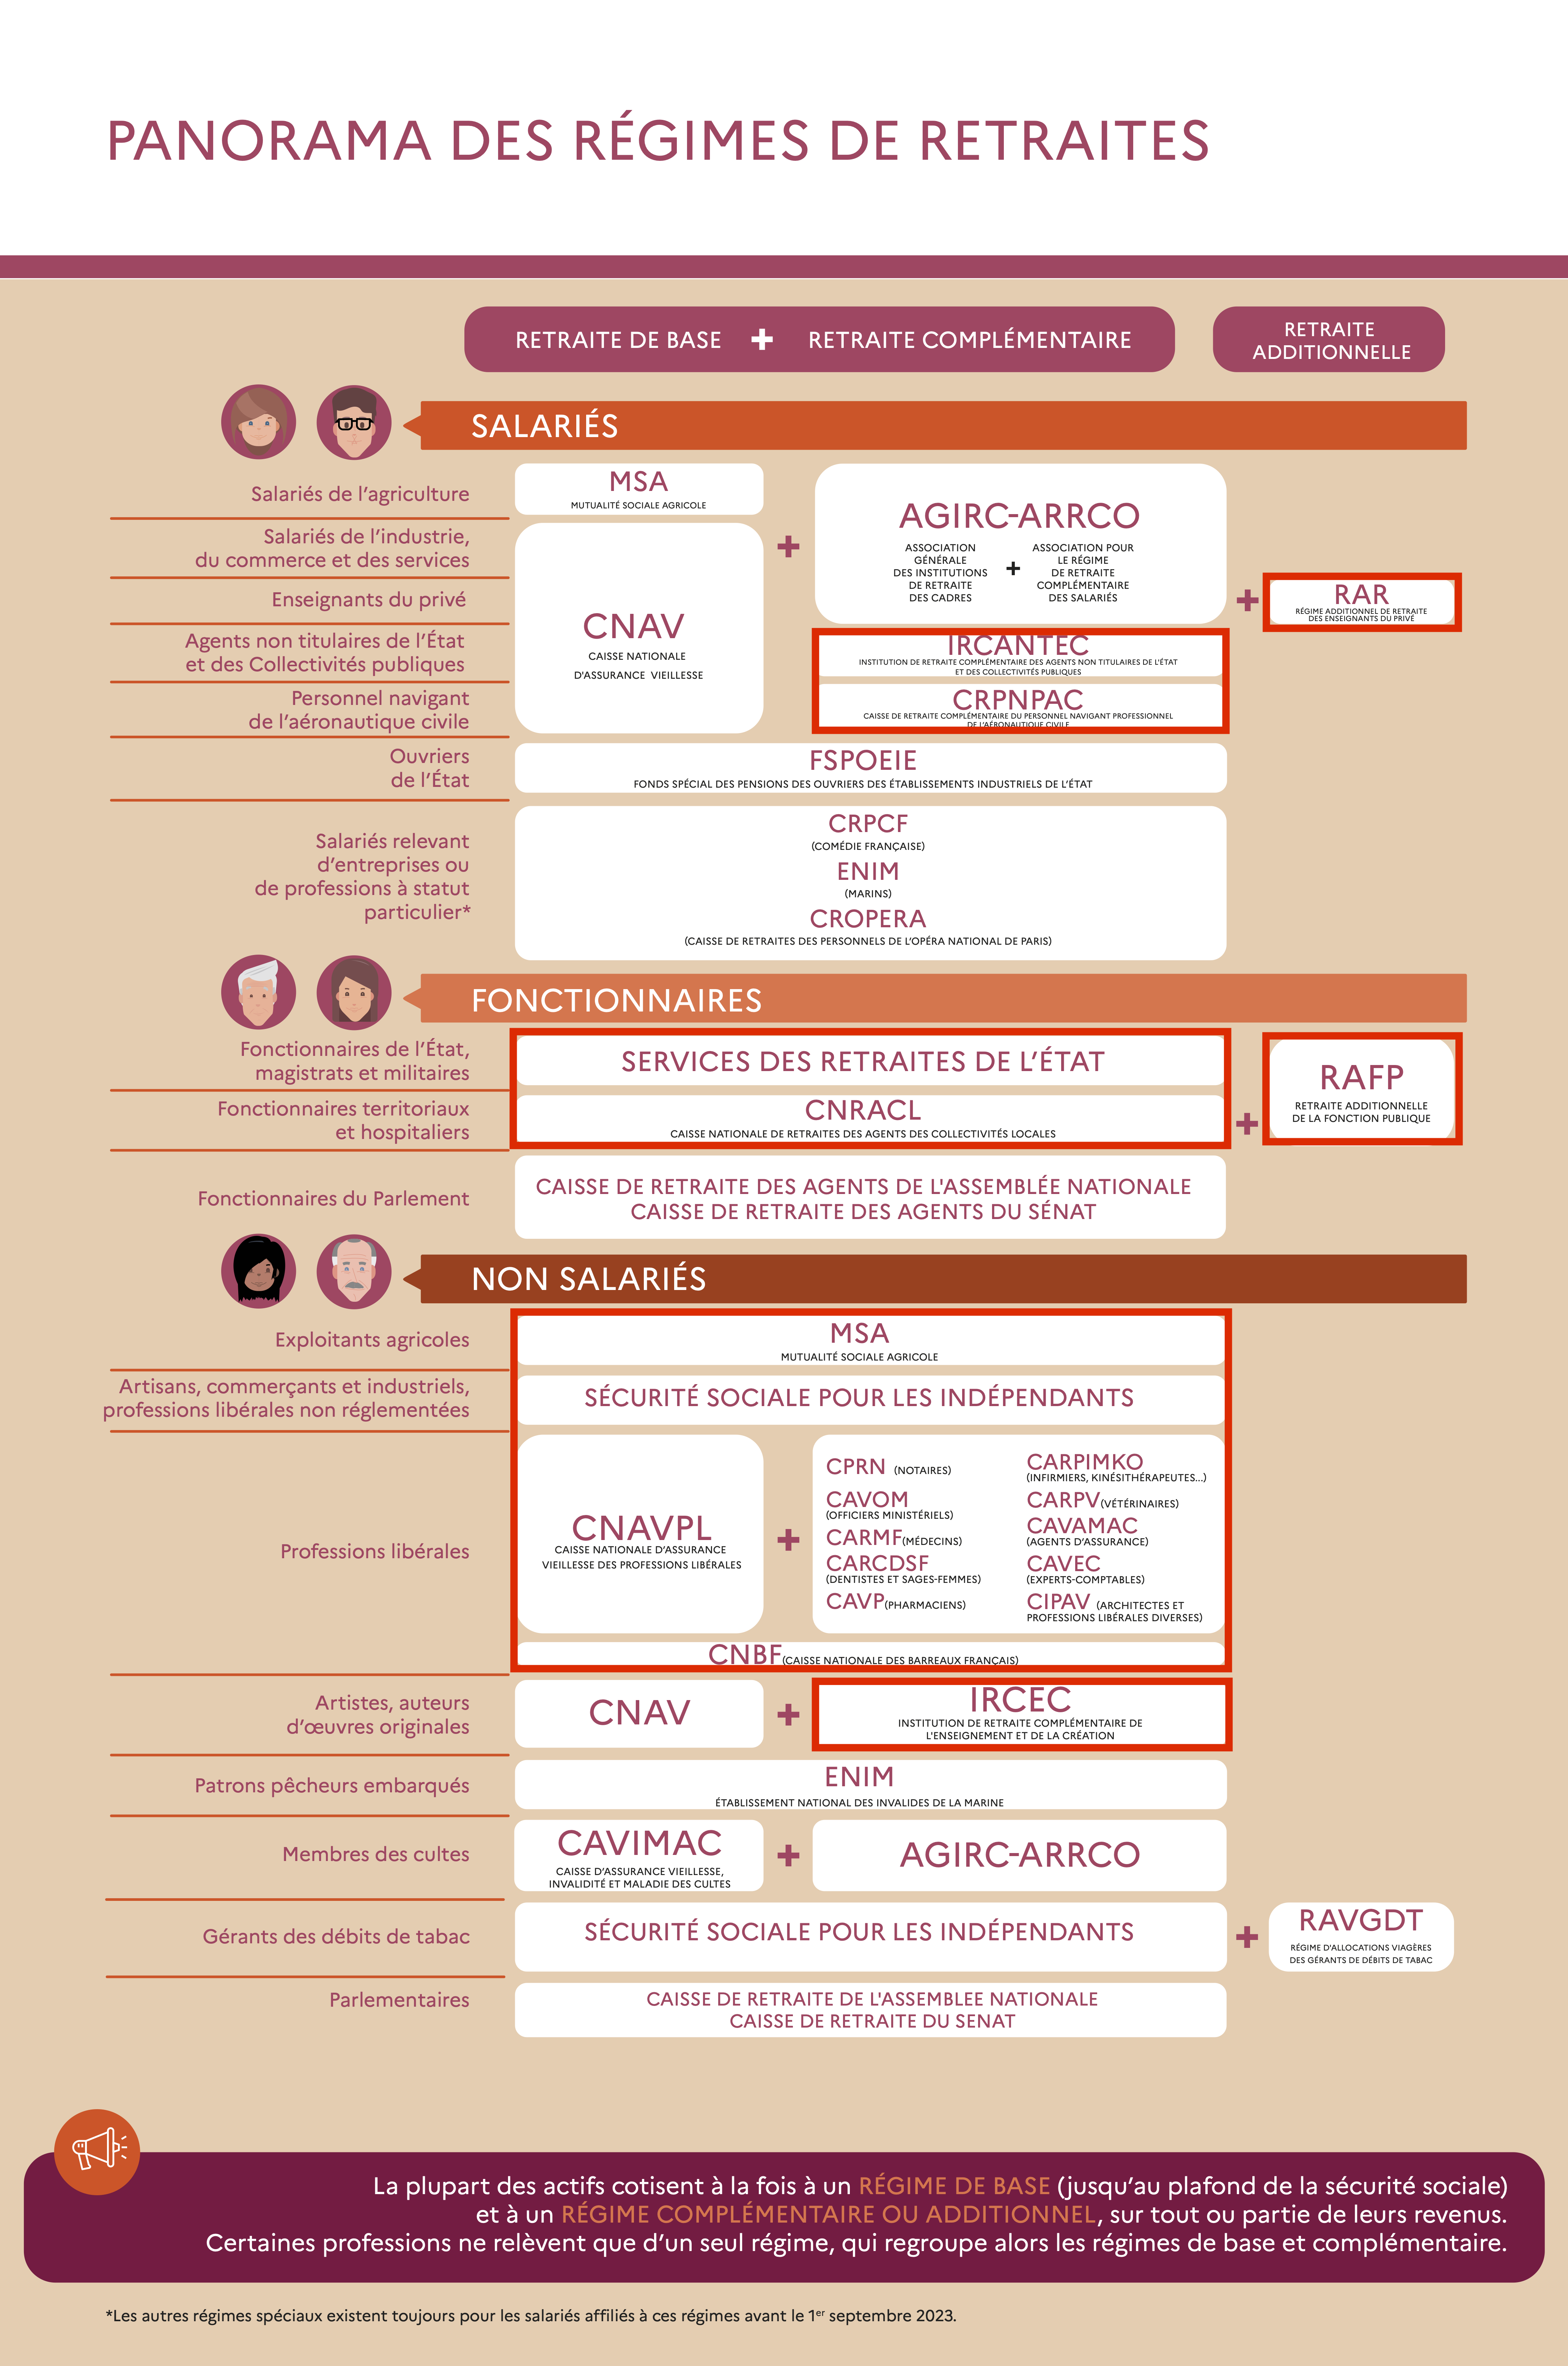
\includegraphics[scale=0.075, keepaspectratio]{figures/chap1/panorama_regimes_retraites.png}
\end{center}

\vspace{-0.5cm}

Ce bureau est donc placé au cœur des problématiques actuelles en matière des frais de santé (PSC) et retraite.

Le bureau 3C est responsable de la tutelle des régimes de son périmètre, ce qui englobe plusieurs aspects importants. L'étendue de son intervention dépend du rôle défini par les textes législatifs pour l'autorité de tutelle. Étant donné que ces régimes complémentaires sont liés à une profession donnée, ils sont co-gérés par les partenaires sociaux. La tutelle de la DSS sur ces régimes se traduit par la signature de conventions d’objectifs et de gestion (COG). Le bureau 3C assure le suivi des ces COG pour les différentes caisses et régimes dont il est responsable.

Premièrement, le bureau 3C est chargé d'assurer la cohérence des textes législatifs entre le régime générale et les complémentaires. Cela inclut, par exemple, la mise en œuvre du relèvement de l'âge de départ à la retraite en vertu de la loi du 9 novembre 2010 portant réforme des retraites. 
Deuxièmement, le bureau exerce un contrôle de légalité sur les décisions prises par les conseils d'administration des caisses, tout en étant responsable de l'évolution de la réglementation des régimes et du bon fonctionnement des caisses.
Enfin, l'une des missions principales du bureau 3C est de garantir la pérennité financière des différents régimes de retraite placés sous sa tutelle. Lorsque le régime est de nature réglementaire, c'est-à-dire que ses paramètres sont fixés par décret, le bureau est à l'initiative des changements de paramètres. Lorsque c'est nécessaires, il est alors chargé de proposer des mesures concertées avec les partenaires sociaux. Cela nécessite non seulement une expertise juridique, mais aussi l'intervention des actuaires à deux niveaux : d'abord pour évaluer l'impact financier des mesures et leur effet sur les assurés, ensuite pour simplifier les propositions et faire preuve de pédagogie lors de la mise en œuvre des réformes, tant auprès des gestionnaires des régimes que des cabinets ministériels.

La gouvernance des caisses de retraite est assuré par des commissions qui portent des noms différentes en fonctions de caisses mais partageant globalement les mêmes objectifs. Le rôle de tutelle du bureau s'incarne notamment pendant ces commissions. Nos collègues du pôle retraite sont chargés de suivre les commissions réglementaires traitant des évolutions des textes juridiques concernant les caisses. Tandis que les membres du pôle actuariat, dont je fais partie, sont chargés de suivre les commissions financières. Celles-ci traitent des sujets relatifs à la gestion financières des caisses (problématiques SI, paramètre du régime, performances des réserves, charte d'investissement éthique, etc.). Notre rôle est de rendre un avis consultatif sur ces sujets et d’apprécier les rapports techniques actuarielles que les caisses ont la charge de présenter annuellement à la tutelle.

Outre cette mission de tutelle et de suivi financier des caisses de retraites, le pôle actuariat a d'autres missions. Une grande partie de son temps est dédié à l'analyse, au chiffrage, puis à la calibration de différentes réformes.
Une autre mission importante est l'analyse et la synthèse des études actuarielles fournies par les régimes dont on assure la tutelle. Enfin il nous arrive de devoir accompagner des missions d'audit de la Cour des comptes et de l'IGAS.

Sur la fin de l'année 2023 et l'année 2024, le pôle Actuariat a été très impliqué dans le suivi de deux projets de politique publique d'envergure : le Sac à dos social de la RATP et la réforme de l'assiette sociale des travailleurs indépendants et des professions libérales. 

L’objet de ce mémoire est d’exposer le contexte de ces réformes et d’expliquer leurs différentes étapes. A la date de remise de ce mémoire, les modalités de fonctionnement du Sac à dos social font encore l'objet d’arbitrage interministériel.
En ce qui concerne la réforme de l’assiette sociale des travailleurs indépendants et des professions libérales, le décret d'application principale a été publié le 5 juillet. Il est intitulé Décret n° 2024-688 du 5 juillet 2024 fixant les modalités de calcul des cotisations et contributions sociales des travailleurs indépendants.